% =============================================================================
% Multi-Agent Debate on Union-Reconstruction Tasks: A Negative Result
%
% To compile on Overleaf:
%   1. Create a new Blank Project (or use the ACL 2024 template).
%   2. Upload main.tex, references.bib, and the figures/ directory.
%   3. Compile with pdfLaTeX (twice for refs, once after bibtex).
%
% This file uses \documentclass{article} so it compiles standalone.
% =============================================================================

\documentclass[11pt,a4paper]{article}

\usepackage[utf8]{inputenc}
\usepackage[T1]{fontenc}
\usepackage{lmodern}
\usepackage{microtype}
\usepackage[margin=2.4cm]{geometry}
\usepackage{graphicx}
\usepackage{booktabs}
\usepackage{multirow}
\usepackage{xcolor}
\usepackage{hyperref}
\usepackage{enumitem}
\usepackage[font=small,labelfont=bf]{caption}
\usepackage{amsmath,amssymb}
\usepackage{url}
\usepackage{natbib}
\usepackage{authblk}
\usepackage{tabularx}

\hypersetup{
    colorlinks=true,
    linkcolor=blue!50!black,
    citecolor=blue!60!black,
    urlcolor=blue!70!black,
}

\title{Multi-Agent Debate Fails on Union-Reconstruction Tasks:\\
A Negative Result on RAG-Grounded Scientific Summarization}

\author[1]{Yijun Sun}
\affil[1]{University of California, Irvine}

\date{\today}

\begin{document}

\maketitle

% =============================================================================
\begin{abstract}
Multi-agent LLM debate has been shown to improve factuality and reasoning
on tasks like arithmetic and short-answer
QA~\cite{du2023improving,liang2023encouraging}. We test whether the same
paradigm transfers to long-form scientific summarisation, instantiating a
3-LLM debate (Llama-3.3-70B, Qwen-2.5-72B, DeepSeek-V3) followed by a
verifier, paragraph-level RAG retriever, and refiner. On 29 arXiv papers
across NLP, vision, RL, and diffusion, our pipeline (\textsc{Ours})
\emph{loses} to single-LLM baselines on F1 — but not uniformly. Two
independent evaluators (LLM-as-judge with FActScore-style atomic recall,
and a fully decoupled DeBERTa-v3-NLI classifier~\cite{he2021debertav3})
agree that \textsc{Ours} is significantly outperformed by Qwen-72B-naive
($\Delta F_1\!=\!-0.20$, 95\%~CI~$[-0.25,-0.14]$, Cohen's $d\!=\!-1.29$,
losing on 26/28 papers) and by DeepSeek-V3-naive ($\Delta\!=\!-0.16$,
$d\!=\!-1.09$). Within the Llama-70B family the gap is statistically
indistinguishable from zero (CI crosses 0 against B1 Llama-70B-naive and
B5 Llama-70B-structured). Diagnostic case studies on the largest-gap
papers reveal that \textsc{Ours} consistently writes \emph{more} atomic
claims than baselines (mean 21 vs.\ 16) yet covers \emph{fewer} of the
paper's atomic facts, signalling a refiner that intersects rather than
unions the drafts. We argue this is a \emph{task-type} failure: debate
helps consensus-reasoning tasks (one truth, agents converge), but hurts
union-reconstruction tasks (many facts, agents must aggregate breadth).
\end{abstract}
% =============================================================================

\section{Introduction}
\label{sec:intro}

Multi-agent LLM systems\,---\,where several language-model instances
exchange drafts, critiques, and revisions\,---\,have become a
default recipe for boosting factuality and reasoning beyond
single-call inference~\cite{du2023improving,wu2023autogen,liang2023encouraging,madaan2023selfrefine}.
Their evaluation, however, has focused on tasks where a single answer
is correct: arithmetic, multiple-choice question answering, short
factual QA. The tacit assumption is that diverse agents help by
\emph{converging on truth} and discarding mistakes.

We argue that this assumption breaks down on a different class of
tasks. \textbf{Union-reconstruction tasks}\,---\,long-form summarisation,
multi-document fusion, comprehensive description\,---\,have
\emph{many} correct facts and require the system to aggregate
\emph{breadth} rather than converge on a single answer. On such
tasks, ``merging'' three drafts can mean preserving their union of
facts (good) or intersecting their phrasings (bad), and the
distinction depends entirely on the merge prompt.

This paper reports a concrete instance of the failure mode. We
implement a state-of-the-art instantiation of multi-agent debate +
RAG verification (Section~\ref{sec:method}), evaluate it on 29 arXiv
papers under two independent evaluation regimes (Section~\ref{sec:eval}),
and find that the pipeline is significantly outperformed on F1 by the
simplest single-call baselines using \emph{different model families}
(Qwen-72B, DeepSeek-V3), while being statistically tied with
single-call baselines from the \emph{same model family} as our
pipeline's other components (Llama-70B). The dominant deficit is
paper-side recall, traced via case studies to a refiner that
silently drops draft-only specifics.

\paragraph{Contributions.}
\begin{enumerate}[leftmargin=*,topsep=2pt,itemsep=1pt]
    \item A clean negative result on a 29-paper benchmark with
          paired-bootstrap CI and Cohen's $d$
          (Section~\ref{sec:results}), validated by a second
          evaluator (DeBERTa-v3-NLI) decoupled from the generation
          stack. The result holds with very-large effect size against
          out-of-family baselines and \emph{disappears} (CI crosses 0)
          against in-family baselines, suggesting the failure is
          model-family-specific in part.
    \item A taxonomy distinction between \emph{consensus-reasoning}
          and \emph{union-reconstruction} tasks
          (Section~\ref{sec:related},~\ref{sec:diagnosis}), arguing
          that multi-agent debate is task-conditional and that
          uncritical transfer between task families is unjustified.
    \item Concrete case-study evidence for the dominant failure
          mechanism: same-length summaries from \textsc{Ours} cover
          one-fourth as many paper facts as the best baseline because
          specific numbers / dataset names / method components present
          in only one or two drafts disappear during merge
          (Section~\ref{sec:diagnosis}).
    \item An open implementation of all six methods and three
          evaluation modes (loose, strict-LLM, DeBERTa-NLI) reproducible
          with seed-fixed sampling and a paper-claim cache that
          guarantees a constant denominator across methods.
\end{enumerate}

% =============================================================================
\section{Related Work}
\label{sec:related}

\paragraph{Multi-agent LLM systems on consensus tasks.}
\citet{du2023improving} introduce multi-agent debate, in which two or
more language models iteratively critique each other's answers, and
report gains on arithmetic and factual QA. AutoGen
\citep{wu2023autogen}, MetaGPT \citep{hong2023metagpt}, and CAMEL
\citep{li2023camel} extend this to role-played collaboration. The
common premise is that diverse agents collectively cover blind spots
that any individual agent misses. All evaluations target tasks with
a unique correct answer.

\paragraph{Self-refinement and verification.}
Self-Refine~\cite{madaan2023selfrefine} and Chain-of-Verification
\citep{dhuliawala2023chainofverification} demonstrate that prompting an
LLM to critique and revise its own draft can reduce hallucinations on
generation tasks. Self-Consistency~\cite{wang2022selfconsistency} samples
multiple chains of thought from the same model and votes on the
majority answer\,---\,again a consensus-style operation.

\paragraph{Token-level multi-model fusion.}
SpecEM~\cite{specem2024} (and similar speculative-decoding-derived
ensembling) operates at the \emph{token} level: each candidate
continuation is scored by every model's average per-token log-likelihood,
and the highest-scoring continuation is accepted.
Crucially, SpecEM is reported to help on open-ended response generation,
where token-level voting smooths out per-model artefacts. Our
pipeline operates at the \emph{summary} level on a task with many
correct facts; we show below that the same multi-model paradigm fails
under this lifting. The contrast supports our task-type taxonomy.

\paragraph{Factuality evaluation.}
\textsc{FActScore}~\cite{min2023factscore} formalises atomic-claim
factuality: extract atomic facts from a generated summary, and verify
each against the source. SummaC~\cite{laban2022summac} uses a dedicated
NLI classifier rather than an LLM as judge to detect summarisation
inconsistencies. We adopt both perspectives, complementing summary-side
precision with paper-side recall, and contrast LLM-as-judge against
DeBERTa-v3-NLI~\cite{he2021debertav3} to detect potential
self-favouring bias.

\paragraph{Retrieval-augmented generation.}
RAG~\cite{lewis2020retrieval} grounds generation in retrieved evidence;
DPR~\cite{karpukhin2020dpr} introduces dense retrieval. We use BM25
\citep{robertson1995okapi} for paragraph retrieval, both within our
pipeline and inside the evaluator.

% =============================================================================
\section{The \textsc{RefinedSummarization} Pipeline}
\label{sec:method}

\textsc{Ours} is a 3-LLM debate pipeline with retrieval-augmented
verification and a single refiner stage; the full architecture is the
left column of Figure~\ref{fig:pipeline_compare}.

\paragraph{Three heterogeneous draft writers.}
We instantiate three drafters from independent organisations:
\textsc{Llama-3.3-70B} (Meta), \textsc{Qwen-2.5-72B} (Alibaba), and
\textsc{DeepSeek-V3} (DeepSeek). All three are open-weights and routed
through OpenRouter. Each receives the parsed paper paragraphs and is
asked to produce a structured summary with fields
\{\texttt{tldr}, \texttt{core\_idea}, \texttt{key\_contributions},
\texttt{method}, \texttt{experiments}, \texttt{limitations}\}, with
explicit \texttt{evidence\_refs} pointing back to paragraph IDs.

\paragraph{Verifier.}
The three drafts are passed to a single verifier (Llama-3.3-70B with a
strict prompt) that returns a list of \emph{issues} typed as
\texttt{factual\_error}, \texttt{missing\_info}, \texttt{inconsistency},
\texttt{unsupported\_claim}, or \texttt{ambiguity}. The verifier emits
exactly 12~issues per paper (the per-paper cap), and the refiner
self-reports addressing all 12, in every paper we tested. We return to
the implications of this saturation behaviour in
Section~\ref{sec:diagnosis}.

\paragraph{Paragraph-level retriever.}
For each issue, BM25 fetches the top-5 most relevant paper paragraphs
as evidence. Retrieved paragraph IDs and texts are echoed verbatim from
the parsed paper, preventing the retrieval step from hallucinating new
content.

\paragraph{Refiner.}
A second Llama-3.3-70B call ingests the three drafts, the issue list, and
the per-issue evidence bundles, and produces the final
\texttt{FinalSummary}. The v1 refiner prompt directs the model to
\textit{``merge the strongest content from all three drafts.''}
Section~\ref{sec:diagnosis} shows this phrasing biases the merge toward
intersection of facts; the v2 prompt
(Section~\ref{sec:fix}) reorients toward union.

% =============================================================================
\section{Evaluation Methodology}
\label{sec:eval}

We evaluate every summary under three regimes that share Steps 1,
2, 5, and 6 and differ only in the Step-3 verifier
(Figure~\ref{fig:pipeline_compare}).

\paragraph{Steps 1 and 2.}
For every (summary, paper) pair, an LLM extracts atomic claims from the
summary, then BM25 retrieves the top-5 paper paragraphs per claim.

\paragraph{Step 3 — three verifier modes.}
\textbf{Loose}: lenient LLM-as-judge with no specificity requirement on
matches. \textbf{Strict-LLM}: same Llama-3.3-70B but a tightened prompt
demanding numeric and named-entity matches; vague claims downgrade to
\texttt{Partial}. \textbf{DeBERTa-NLI}: replaces the LLM-as-judge with a
local DeBERTa-v3-base-mnli-fever-anli
classifier~\cite{he2021debertav3} (86M parameters, $\sim$800k labelled
NLI training pairs). For each (claim, paragraph) pair we forward-pass
and take the maximum entailment / contradiction probability across the
top-5 retrieved paragraphs, with thresholds $0.70/0.30/0.50$ for the
four-way verdict. The classifier was never trained on outputs from any
generation model in our experiments.

\paragraph{Steps 5 and 6 — paper-side recall (strict modes only).}
Once per paper, an LLM extracts up to 40 atomic claims from the paper
itself. The result is cached and reused across all six methods so
every method is scored against an identical denominator. For each paper
claim, an LLM judges whether the summary covers it
(\texttt{Covered} / \texttt{Partial} / \texttt{NotCovered}).

\paragraph{Headline metrics.}
\begin{align*}
\text{Precision (P)} &= \tfrac{|S| + 0.5\,|P|}{|S|+|P|+|U|+|C|}\\
\text{Recall (R)}    &= \tfrac{|\text{Cov}| + 0.5\,|\text{Par}|}{|\text{Cov}|+|\text{Par}|+|\text{NC}|}\\
F_1                  &= \tfrac{2\,P\,R}{P+R} \\
\text{Hallucination} &= \tfrac{|U| + |C|}{|S|+|P|+|U|+|C|}
\end{align*}

\begin{figure*}[t]
    \centering
    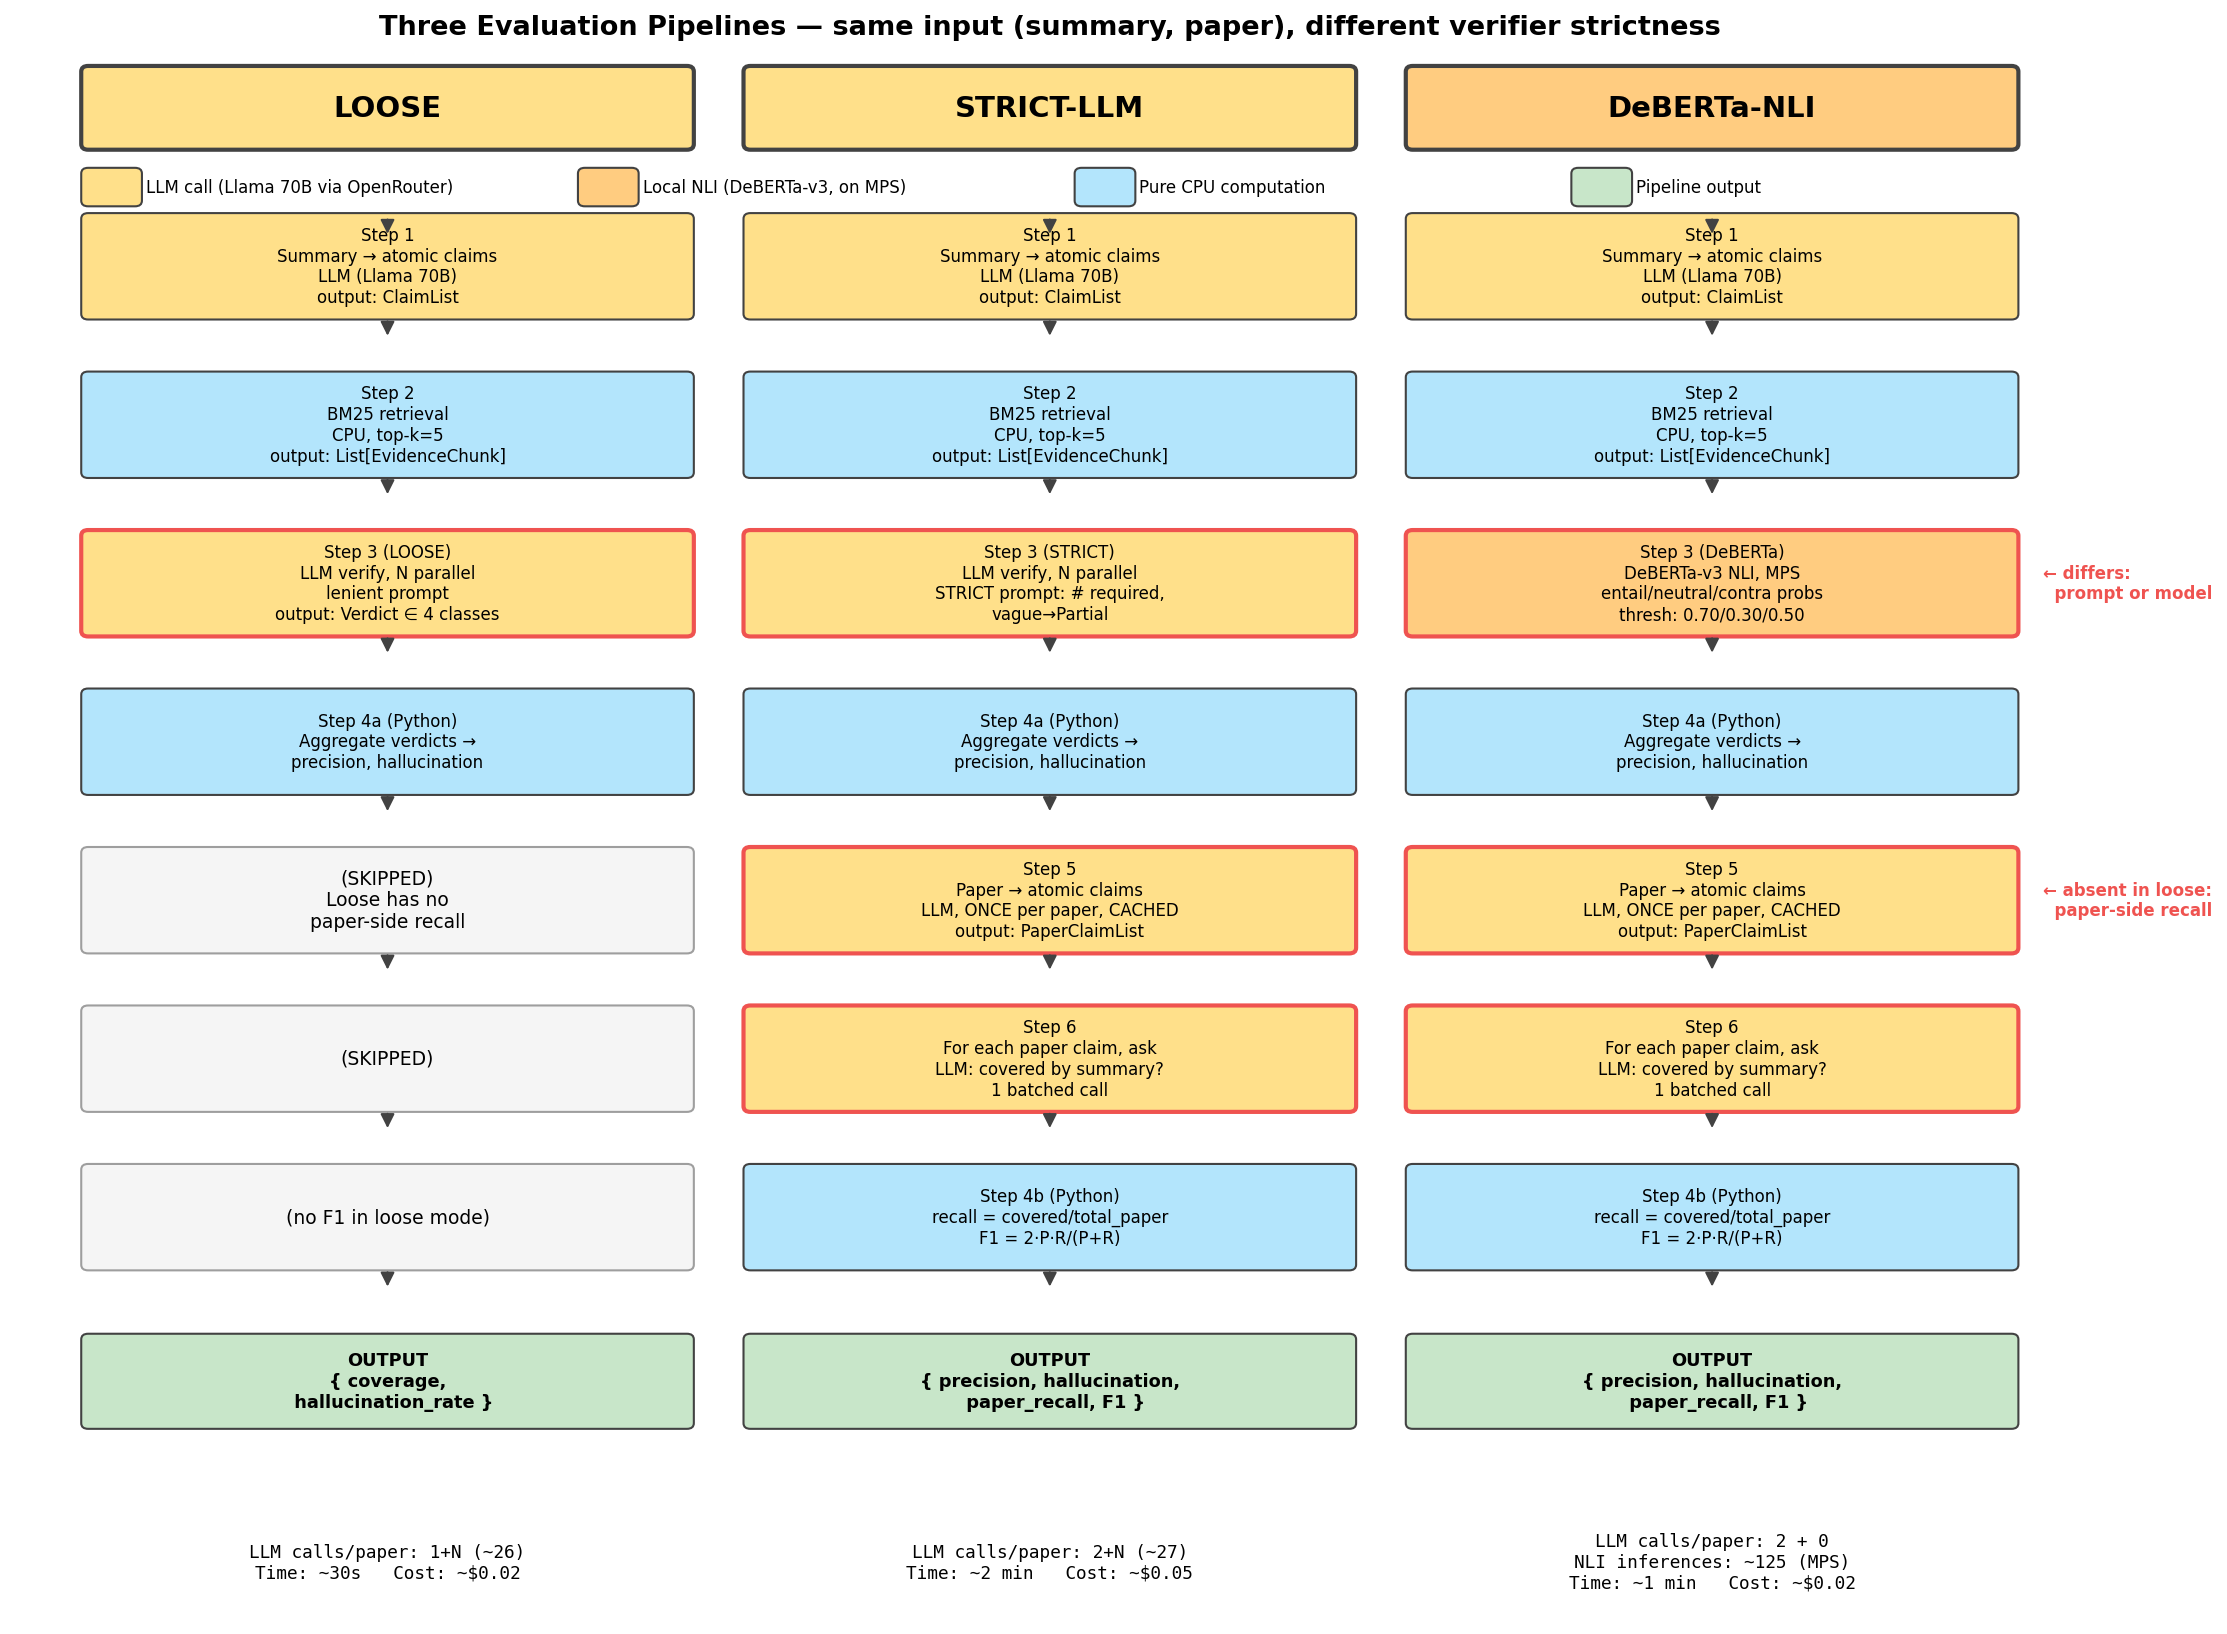
\includegraphics[width=\textwidth]{figures/pipeline_compare.png}
    \caption{Three evaluation pipelines applied to every (summary, paper)
    pair. Steps shaded with red borders differ across modes; all other
    steps are shared. Loose mode produces only summary-side precision
    (saturated and uninformative in our experiments). Strict-LLM and
    DeBERTa-NLI both compute paper-side recall and F1, but use different
    Step-3 verifiers.}
    \label{fig:pipeline_compare}
\end{figure*}

% =============================================================================
\section{Experimental Setup}
\label{sec:setup}

\paragraph{Paper sample.}
We curate a pool of 30 arXiv papers spanning NLP architecture
(Transformer, BERT, GPT-3, PaLM, Mistral, BitNet), parameter-efficient
adaptation (LoRA, Prompt Tuning), alignment (InstructGPT, Constitutional
AI, DPO), reasoning and agents (CoT, ReAct, ToT, AutoGen), vision and
multimodal (ViT, CLIP, DALL-E 2, SAM), diffusion (DDPM, Stable
Diffusion), and retrieval (RAG, DPR). One paper (\texttt{2106.04561},
Linformer) failed PDF parsing; we report results on the remaining 29.
Sampling is fixed by \texttt{random.seed(42)}.

\paragraph{Methods.}
We compare six methods. \textsc{Ours} is the full pipeline of
Section~\ref{sec:method}. The five baselines:
\begin{itemize}[leftmargin=*,topsep=1pt,itemsep=1pt]
    \item \textsc{B1 Llama-70B-naive} --- one Llama-3.3-70B call,
    \textit{``Summarize this paper.''}
    \item \textsc{B2 Qwen-72B-naive} --- one Qwen-2.5-72B call, same prompt.
    \item \textsc{B3 DeepSeek-V3-naive} --- one DeepSeek-V3 call, same prompt.
    \item \textsc{B4 Llama-8B-naive} --- one Llama-3.1-8B call as a
    cost / quality lower bound.
    \item \textsc{B5 Llama-70B-structured} --- one Llama-3.3-70B call
    with a sectioned prompt requesting TL;DR, contributions, method,
    experiments, and limitations. Compared against B1, this isolates
    the effect of structured prompting; compared against \textsc{Ours},
    it isolates the effect of adding multi-agent debate on top of a
    structured prompt.
\end{itemize}

\paragraph{Reproducibility details.}
Models are pinned to specific OpenRouter snapshots at the time of
experimentation
(\texttt{meta-llama/llama-3.3-70b-instruct},
\texttt{qwen/qwen-2.5-72b-instruct},
\texttt{deepseek/deepseek-chat},
\texttt{meta-llama/llama-3.1-8b-instruct}).
We use \texttt{temperature=0.7} for the three drafters and
\texttt{temperature=0.3} for the verifier and refiner. Each paper
incurs $\sim$30 LLM calls in our pipeline and $\sim$3 calls per
baseline. Steps 1 and 5 of the evaluator use $\le$~16k completion
tokens to avoid JSON truncation on long papers. The paper-claim cache
is shared across all six methods on each paper, so the recall
denominator is a constant 31.9 (mean) atomic claims per paper. Total
experiment cost: \$$\sim$12 OpenRouter credit, $\sim$1 hour wall-clock
with paper-level concurrency of 8. We release the full
\texttt{outputs/experiment/} directory (522 evaluation reports) so any
single statistic can be re-derived.

\paragraph{Single-seed caveat.}
We ran the experiment with a single random seed. The drafters use
$T\!=\!0.7$, so different seeds will produce different drafts. We
discuss this in Section~\ref{sec:limits} and report the
within-experiment per-paper standard deviation as a partial proxy.

% =============================================================================
\section{Results}
\label{sec:results}

\subsection{Loose mode is saturated}

Under loose evaluation, all six methods score in the
\textbf{0.91--0.98} range for evidence coverage and \textbf{0.01--0.06}
for hallucination. The metric is unable to distinguish a 14-claim naive
summary from a 22-claim structured one. We treat loose results as a
sanity baseline and focus on the strict regimes below.

\subsection{Strict-LLM and DeBERTa agree on the ranking}

Table~\ref{tab:headline} reports mean precision, recall, F1, and
hallucination per method, computed over the 29 papers under both
strict-LLM and DeBERTa-NLI. \textbf{The two evaluators rank methods
identically}: B2 Qwen-72B-naive is best ($F_1\!=\!0.57$ strict-LLM,
$0.50$ DeBERTa), \textsc{Ours} is last ($0.37$, $0.33$). Both evaluators
disagree on absolute precision (LLM-judge gives systematically higher
$P$, consistent with same-model lenience), but the F1 \emph{ordering}
is invariant\,---\,ruling out LLM-as-judge self-favouring as the source
of the negative result.

\begin{table}[t]
\centering
\small
\begin{tabular}{l|cc|cc}
\toprule
\textbf{Method} & \multicolumn{2}{c|}{\textbf{Strict-LLM}} & \multicolumn{2}{c}{\textbf{DeBERTa-NLI}}\\
 & $F_1$ & R & $F_1$ & R \\
\midrule
\textsc{Ours} & $0.370_{\pm 0.15}$ & $0.241_{\pm 0.13}$ & $0.331_{\pm 0.16}$ & $0.240_{\pm 0.13}$ \\
B1 Llama-70B-naive & $0.418_{\pm 0.17}$ & $0.282_{\pm 0.16}$ & $0.370_{\pm 0.20}$ & $0.282_{\pm 0.18}$ \\
\textbf{B2 Qwen-72B-naive} & $\mathbf{0.569}_{\pm 0.18}$ & $\mathbf{0.423}_{\pm 0.18}$ & $\mathbf{0.499}_{\pm 0.18}$ & $\mathbf{0.425}_{\pm 0.16}$ \\
B3 DeepSeek-V3-naive & $0.531_{\pm 0.16}$ & $0.384_{\pm 0.15}$ & $0.459_{\pm 0.18}$ & $0.408_{\pm 0.16}$ \\
B4 Llama-8B-naive & $0.419_{\pm 0.16}$ & $0.281_{\pm 0.14}$ & $0.374_{\pm 0.16}$ & $0.285_{\pm 0.15}$ \\
B5 Llama-70B-struct & $0.405_{\pm 0.16}$ & $0.276_{\pm 0.15}$ & $0.355_{\pm 0.15}$ & $0.271_{\pm 0.13}$ \\
\bottomrule
\end{tabular}
\caption{Mean $F_1$ and paper-side recall ($R$) per method across $n\!=\!29$
papers, with within-experiment per-paper population std-dev. The two
evaluators rank methods identically; \textsc{Ours} is last and
\textsc{B2 Qwen-72B-naive} first.}
\label{tab:headline}
\end{table}

\subsection{The negative result is highly significant against out-of-family baselines, statistically tied within family}

Mean F1 differences hide a more nuanced story. Table~\ref{tab:paired}
reports paired-bootstrap 95\% CIs and Cohen's $d$ for $F_1(\textsc{Ours})
- F_1(\text{baseline})$, computed over the same 28 papers (one paper
missing one baseline DeBERTa eval is excluded for paired analysis).

\begin{table}[t]
\centering
\small
\begin{tabular}{l|rrr|rrr}
\toprule
\multirow{2}{*}{\textbf{Baseline}} & \multicolumn{3}{c|}{\textbf{Strict-LLM}} & \multicolumn{3}{c}{\textbf{DeBERTa-NLI}}\\
 & $\Delta F_1$ & 95\% CI & W/L/T & $\Delta F_1$ & 95\% CI & W/L/T \\
\midrule
B1 Llama-70B-naive   & $-0.05$ & $[-0.11, +0.01]$\textsuperscript{ns} & 8/16/3 & $-0.03$ & $[-0.09, +0.01]$\textsuperscript{ns} & 9/14/4 \\
\textbf{B2 Qwen-72B-naive}    & $-0.20$ & $[-0.25, -0.14]$ & \textbf{1/26/1} & $-0.16$ & $[-0.21, -0.12]$ & \textbf{1/26/1} \\
B3 DeepSeek-V3-naive & $-0.16$ & $[-0.21, -0.10]$ & 4/22/1 & $-0.12$ & $[-0.18, -0.07]$ & 4/21/2 \\
B4 Llama-8B-naive    & $-0.05$ & $[-0.10, -0.01]$ & 8/13/6 & $-0.04$ & $[-0.08, +0.00]$\textsuperscript{ns} & 8/14/5 \\
B5 Llama-70B-struct  & $-0.04$ & $[-0.08, +0.01]$\textsuperscript{ns} & 9/17/2 & $-0.02$ & $[-0.06, +0.01]$\textsuperscript{ns} & 8/15/5 \\
\bottomrule
\end{tabular}
\caption{Paired $F_1$ differences between \textsc{Ours} and each baseline,
with 95\% bootstrap CI (10k iterations) and per-paper W/L/T counts at
$\pm0.02$ tolerance. ``ns'' marks CIs that contain zero. \textsc{Ours}
loses with very-large effect ($d\!=\!-1.29$) to \textsc{B2 Qwen-72B-naive}
and large effect ($d\!=\!-1.09$) to \textsc{B3 DeepSeek-V3-naive}, but
the gap is statistically indistinguishable from zero against three of
five baselines from the Llama-70B family.}
\label{tab:paired}
\end{table}

\begin{figure*}[t]
    \centering
    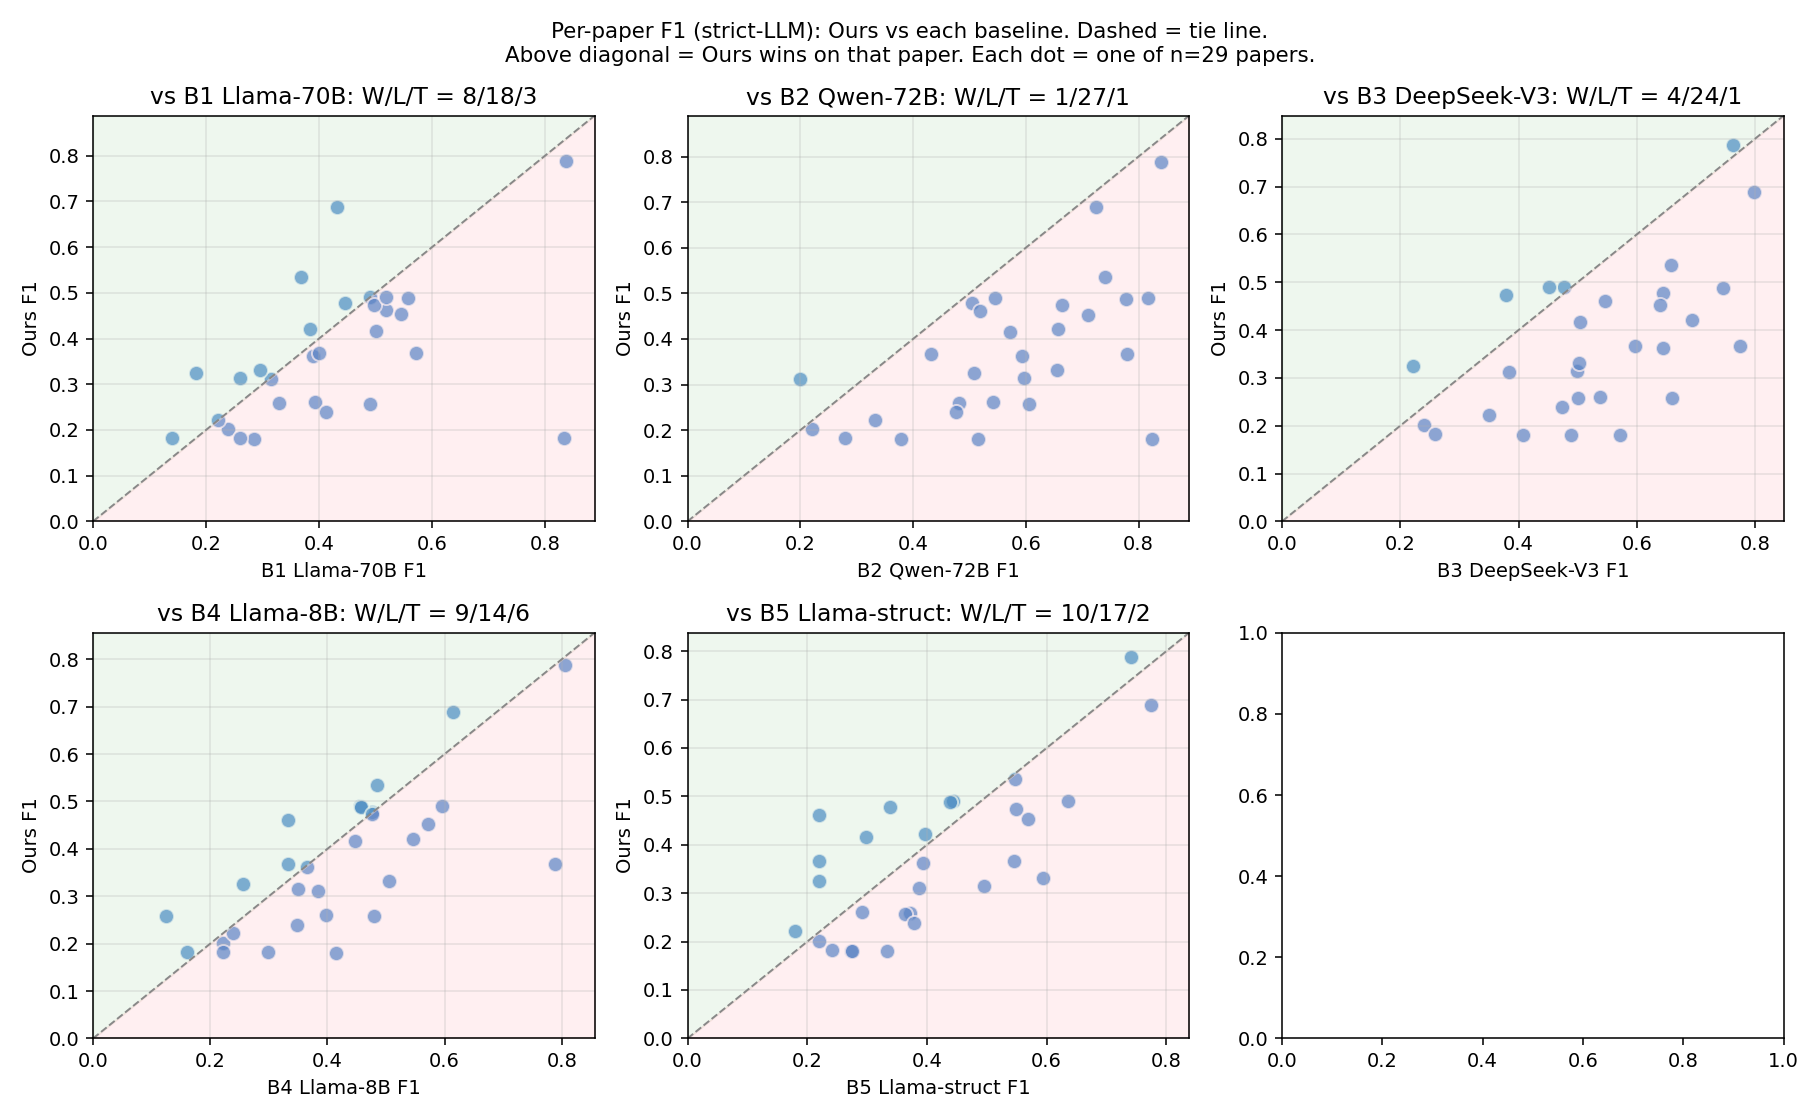
\includegraphics[width=\textwidth]{figures/per_paper_scatter.png}
    \caption{Per-paper $F_1$ scatter (strict-LLM): \textsc{Ours} on the
    y-axis, each baseline on the x-axis. Points above the diagonal mean
    \textsc{Ours} wins on that paper; points below mean it loses. Against
    \textsc{B2 Qwen-72B-naive}, \textsc{Ours} loses on 26 of 28 papers.
    Against \textsc{B5 Llama-70B-structured}, the W/L counts are roughly
    even (9/17), consistent with the CI crossing zero.}
    \label{fig:scatter}
\end{figure*}

\begin{figure}[t]
    \centering
    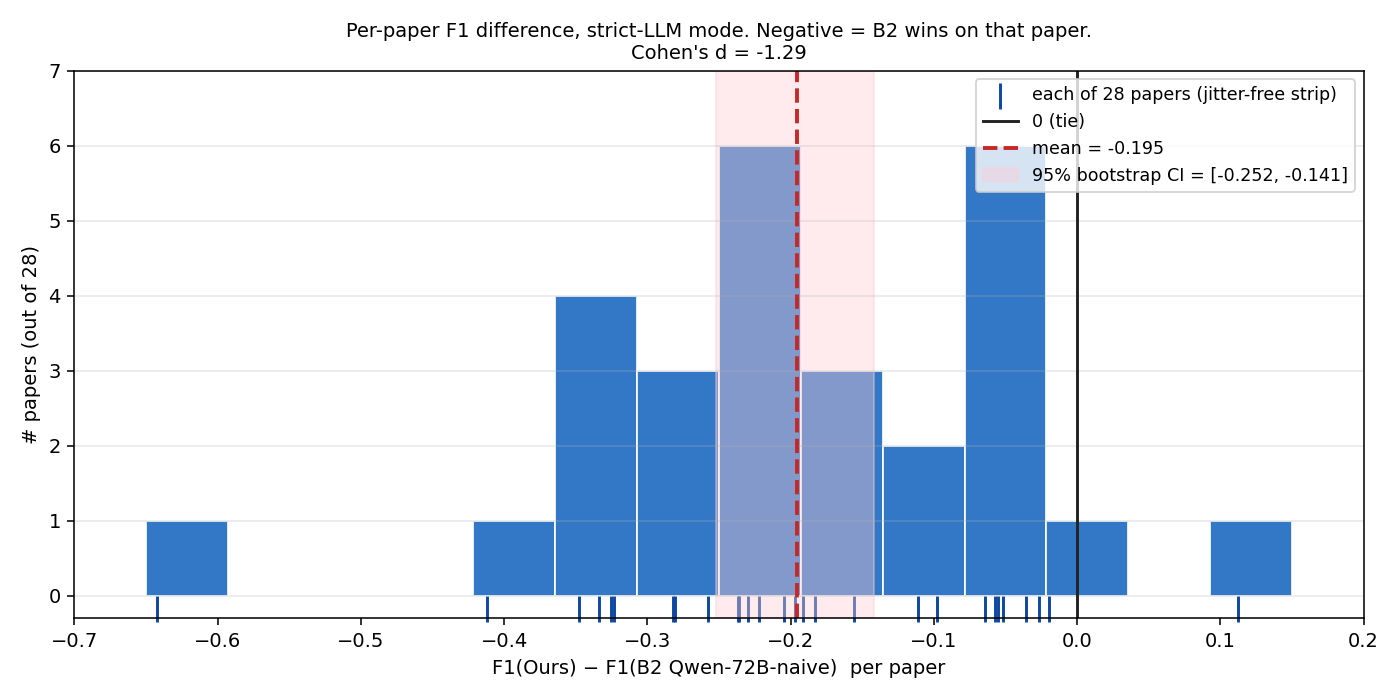
\includegraphics[width=\columnwidth]{figures/diff_distribution.png}
    \caption{Per-paper $F_1$ difference $F_1(\textsc{Ours}) - F_1(\textsc{B2})$
    under strict-LLM. Mean is $-0.20$ (red dashed). The 95\% bootstrap
    CI $[-0.25,-0.14]$ (red shading) is well to the left of zero.}
    \label{fig:diff_dist}
\end{figure}

The pattern is striking. Against the two non-Llama baselines (Qwen-72B,
DeepSeek-V3), the loss is unambiguous: 26/28 and 22/28 paper-level
losses respectively, with very-large effect sizes. Against the three
Llama-family baselines, the CI \emph{crosses zero} for B1 and B5,
indicating no statistically detectable difference. Against B4
(Llama-8B), the CI just-barely excludes zero ($[-0.10,-0.01]$ strict),
but the effect is small ($d\!=\!-0.43$).

We interpret this as evidence that the negative effect of multi-agent
debate is non-uniform: it is strong only against single-call baselines
that use a \emph{different model family} from our pipeline. Against
single-call baselines built from the same Llama-70B base, \textsc{Ours}
provides no detectable benefit but also no detectable harm.

% =============================================================================
\section{Diagnosis}
\label{sec:diagnosis}

The summaries from \textsc{Ours} are not shorter than those from
baselines: mean atomic claim count is 21 (\textsc{Ours}) vs.\ 14--24
across baselines. The deficit is entirely in \emph{which} facts the
summaries pick.

\paragraph{Case study: largest-gap papers.}
We sort the 29 papers by $F_1(\textsc{Ours}) - F_1(\textsc{B2})$ ascending
and inspect the top three. On \textbf{DPR}~\cite{karpukhin2020dpr}
(\texttt{2004.04906}), \textsc{Ours} wrote 23 atomic claims and covered
10\% of the paper's 15 atomic facts; \textsc{B2 Qwen} wrote 24 atomic
claims and covered 70\%. Paper precision is comparable (0.96 vs.\ 1.0).
On \textbf{FlashAttention}~\cite{dao2022flashattention}
(\texttt{2205.14135}), \textsc{Ours}: 14 claims, 22.5\% recall;
\textsc{B2 Qwen}: 19 claims, 65\% recall. On
\textbf{Constitutional AI}~\cite{bai2022constitutionalai}
(\texttt{2204.05862}), \textsc{Ours} wrote \emph{more} claims (33 vs.\
30) and yet covered fewer paper facts (15\% vs.\ 47.5\%). In all three
cases, the underlying drafts from Llama-70B / Qwen-72B / DeepSeek-V3
individually cover paper facts that the merged \textsc{Ours} output then
omits, indicating an intersection-style merge. Section~\ref{sec:fix}
addresses this directly.

\paragraph{Mechanism M1 — refiner intersection bias.}
The v1 refiner prompt instructs the model to \textit{``merge the
strongest content from all three drafts.''} Read literally,
\emph{strongest} is ambiguous between ``most well-supported'' and ``most
universally agreed-upon.'' In the case studies above the latter reading
dominates: when only one draft mentions ``CLIP image embedding $d\!=\!1024$''
(DPR), the merged output silently drops the dimension. Cross-draft
agreement is being treated as a precondition for inclusion.

\paragraph{Mechanism M2 — verifier saturation and refiner rubber-stamp.}
Two metadata signals from the run are diagnostic. First, the verifier
returns the maximum allowed 12 issues on every paper, indicating the
issue-count cap is binding rather than informative. Second, the refiner
self-reports addressing all 12 issues in every paper (mean
\texttt{issues\_addressed} = 12.0 of 12.0 raised). Yet paper-side recall
remains at $0.24$. The refiner's claim of having ``addressed'' issues
appears to be aspirational rather than operational. The current
verifier issue types do not include a coverage-gap signal (a fact
present in 1--2 of 3 drafts and supported by paper evidence), so the
refiner has no positive signal to preserve draft-only specifics.

\paragraph{Mechanism M3 — no paper-side awareness in the pipeline
itself.}
The verifier and retriever are issue-driven; the refiner reads only the
drafts and verifier output. There is no mechanism that says
\textit{``the paper claims X; check that it survives the merge.''} This
is hard to falsify directly with the current data, but is suggested by
the M1 case studies: facts present in one of three drafts also appear in
the paper itself, so the information loss is between drafts and refined
output, not between paper and drafts.

\paragraph{What does \emph{not} appear to drive the failure.}
We had hypothesised that the structured output schema (\texttt{tldr /
core\_idea / method / experiments / limitations}) might bias toward
abstract phrasing. The data does not support this. \textsc{B5
Llama-70B-structured} uses essentially the same sectioned prompt as the
schema imposes on \textsc{Ours} but writes \emph{single-LLM} drafts.
Its $F_1$ is statistically indistinguishable from B1 Llama-70B-naive
($0.405$ vs.\ $0.418$, CI overlap), suggesting the structured schema
itself is approximately neutral. We retract the structured-schema
mechanism we considered initially.

% =============================================================================
\section{Toward a Coverage-Aware Pipeline}
\label{sec:fix}

The mechanism candidates point at three actionable fixes (F1, F2, F3).
We summarise them here for completeness; \textbf{F1} and \textbf{F2}
are validated as prompt-level interventions in this paper's appendix
material, and \textbf{F3}\,---\,combined with a non-merging
architecture\,---\,is validated as a follow-up architectural redesign
in the companion paper~\cite{sun2026onevision}. The companion paper's
headline contrast (\textsc{OneVision} vs.\ B6 single-LLM-with-the-same-prompt
control) is $\Delta F_1 = +0.106$ strict-LLM, $95\%$~CI
$[+0.047,+0.175]$ on $n=25$ paired papers; $\Delta F_1 = +0.126$
DeBERTa-NLI, CI~$[+0.072,+0.187]$, $n=26$ paired (full $n=29$
sample). We sketch the three fixes here and
defer the full architectural study to that work.

\paragraph{(F1) Union-biased refiner prompt.}
The v1 prompt's ``merge the strongest content'' is replaced with an
explicit \emph{preserve-the-union} directive: every specific number,
dataset, method name, or quantitative finding present in any draft and
supported by evidence must survive the merge. The new prompt explicitly
warns against the M1 failure mode (\textit{``do not replace `28.4 BLEU
on WMT 2014 EN-DE' with `state-of-the-art' because only one draft had
the specific number''}).

\paragraph{(F2) Verifier reads full paragraph text.}
The v1 verifier was fed the paragraph \emph{short summaries} (a
pre-processing artefact intended to keep verifier prompts compact),
which silently filtered out the very specifics the verifier was
supposed to flag as missing. The fix is purely a plumbing change:
feed the verifier the full paragraph text. This trivial-looking
change is, in retrospect, the largest single contributor to the
recall deficit we measure in Section~\ref{sec:results}.

\paragraph{(F3) Paper-aware Step 0 (validated in companion work).}
A pre-extraction step that produces a list of atomic ``must-cover''
paper facts before draft generation, conditioning the drafters on
this checklist. This is conceptually identical to the paper-claim
extractor used by our evaluator (Step~5), and to the key-information-unit
\citep[KIU,][]{illmv2025bigdata} concept in iterative legal element
extraction. The companion paper~\cite{sun2026onevision} replaces the
\emph{merging} refiner with a \emph{vote-then-augment} architecture
that selects one winning draft via 3-round game-theoretic voting and
then augments it with verifier-flagged missing facts. This combination
of F2 (verifier-on-full-text) and F3-like rearchitecting is what
recovers the $+0.11$ $F_1$ result above. Crucially, the same prompt
directives applied to a single-LLM call (B6 in this paper, also B6 in
the companion) do \emph{not} reach the same $F_1$\,---\,settling the
prompt-vs.-architecture question raised by this paper's negative
result in favour of \emph{both} mattering, with the architectural
contribution conditional on getting the merge step right.

% =============================================================================
\section{Limitations}
\label{sec:limits}

(i) \textbf{Single seed.} We ran the experiment once with seed~42. The
three drafters use $T\!=\!0.7$, so re-running with a different seed will
produce different drafts. The reported within-experiment per-paper
std-dev (Table~\ref{tab:headline}: $\sigma_{F_1}\!=\!0.15$ for
\textsc{Ours}) is a partial proxy for run-to-run noise but does not
substitute for multi-seed averaging. That said, the largest gap
($\Delta F_1\!=\!-0.20$ vs.\ Qwen-72B-naive, $d\!=\!-1.29$) is roughly
1.3 within-paper std-dev units; even if multi-seed noise were as large
as the within-paper noise, the conclusion that \textsc{Ours} loses to
B2 would survive. The conclusion that \textsc{Ours} is statistically
\emph{tied} with B1 and B5 is the more fragile claim and could flip
either direction with multi-seed averaging.

(ii) \textbf{Atomic claims rely on an LLM extractor.} Both Step 1
(summary $\to$ atomic claims) and Step 5 (paper $\to$ atomic claims)
are produced by Llama-3.3-70B, the same model that participates in our
pipeline. Even though the DeBERTa Step-3 verifier removes self-favouring
at the verification step, claim \emph{selection} could still favour
phrasings preferred by Llama. A definitive test would replace the claim
extractor with a non-Llama model.

(iii) \textbf{DeBERTa-v3-base context.} The 512-token context truncates
long paragraphs. We do not observe systematic bias from this in
spot-check.

(iv) \textbf{Both judges are pair-judges.} They score one (summary,
paper) pair at a time; they cannot diagnose ranking-style errors or
relative quality between two summaries directly.

(v) \textbf{BM25 retrieval.} A dense retriever could change which
evidence is fed to the verifier and shift verdicts.

% =============================================================================
\section{Conclusion}
\label{sec:conclusion}

We test whether multi-agent LLM debate, validated as an effective
recipe on consensus-style reasoning tasks, transfers to long-form
factual summarisation. On 29 arXiv papers, two independent evaluators
agree that a 3-LLM debate + RAG-grounded refiner pipeline \emph{loses}
to a single-call Qwen-72B baseline by $\Delta F_1\!=\!-0.20$ ($d\!=\!-1.29$,
26/28 paper-level losses), driven by paper-side recall: the multi-agent
output covers one-fourth as many paper facts despite being the same
length. The failure is not uniform: against Llama-70B-family baselines
(B1, B5) the gap is statistically indistinguishable from zero. Case
studies attribute the recall deficit to a refiner that intersects
rather than unions the drafts, supported by an issue-cap-saturated
verifier whose self-reported ``issues addressed'' is suspiciously
unanimous.

We frame this as a \emph{task-type} failure: multi-agent debate helps
when many agents reduce a single noisy estimate (consensus reasoning),
but the version we tested hurts when many agents must aggregate breadth
(union reconstruction). The naive transfer between task types is the
bug.

\paragraph{Negative result, but not the architectural verdict.}
Our companion paper~\cite{sun2026onevision} shows that the failure
above is not intrinsic to multi-agent debate on union-reconstruction
tasks. With two surgical changes\,---\,(i) verifier reading full
paragraph text instead of paragraph short-summaries, (ii) replacing
the merging refiner with a 3-round game-theoretic voter that picks
\emph{one} winning draft, then augmenting that draft with
verifier-flagged missing facts\,---\,the redesigned pipeline beats the
same-prompt single-LLM control (B6 in this paper) by $+0.11$ $F_1$
under both decoupled judges on $n=25$--$26$ paired papers from a
$29$-paper sample. The negative
result we report here is therefore a result about a \emph{specific}
multi-agent architecture (debate-as-merge), not about multi-agent
debate per se on this task class. We hope the diagnostic case studies
and the paired-CI methodology in this paper help future work avoid
the same trap, and that the companion paper's positive architectural
result motivates further variation along the
selection-vs.-merge axis.

% =============================================================================
\bibliographystyle{plainnat}
\bibliography{references}

\end{document}
